% tags:[physics,homework]

\documentclass[UTF8]{ctexart} % 使用 ctexart 文档类，自动处理中文

\usepackage{fireinice}
\usepackage{pgfplots}
\pgfplotsset{compat=1.17} % 确保你使用的是最新版本

\title{Physics Homework - Term 1 Week 1}
\author{Ithea}
\date{2026-03-13 17:48:41}

\begin{document}

\maketitle

\section{Class 1}

\begin{question}{T1-1.1}
一物体沿 \(x\) 轴运动，其运动方程为 \(x = 100t - 5t^2\)，式子中 \(x\) 的单位为 m，\(t\) 的单位为 s。
(1) 计算物体在前 3s 内的平均速度，以及在 \(t=3\text{s}\) 时的瞬时速度和加速度。
(2) 画出 \(x-t\) 曲线，并标明在哪段时间内物体速度沿 \(x\) 轴正方向。
\end{question}
\begin{solve}

(1):

\[
\begin{gathered}
\overline v=\dfrac{x(3)-x(0)}{3}=85 m/s \\
v=\dot x=100-10t=70 m/s \\
a=\ddot x=-10 m/s^2
\end{gathered}
\]


(2):

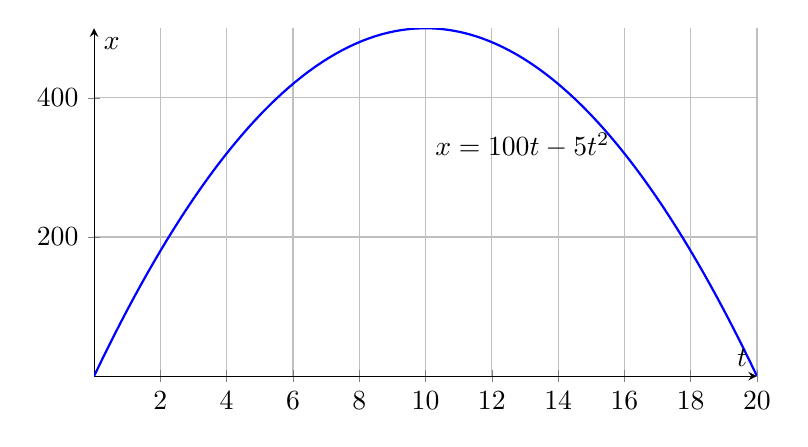
\begin{tikzpicture}
    \begin{axis}[
        axis lines = middle, % 设置坐标轴线在中心
        xlabel = \(t\), ylabel = \(x\),
        ymin=0, ymax=500, % 根据需要调整y轴范围
        xmin=0, xmax=20, % 根据需要调整x轴范围
        domain=0:20, % t的定义域
        samples=100, % 取样点数，数值越大曲线越平滑
        grid=both, % 显示网格
        width=10cm, % 图像宽度
        height=6cm, % 图像高度
        ]
        % 绘制函数图像
        \addplot [blue, thick] {100*x - 5*x^2};
        % 添加标签
        \node at (axis cs:10,300) [anchor=south west] {\(x=100t-5t^2\)};
    \end{axis}
\end{tikzpicture}

\(x<10\)时速度沿\(x\)轴正方向, \(x>10\)时速度沿\(x\)轴负方向.

\end{solve}

\begin{question}{T2-1.3}
两个小球从高度相差 10m 的位置同时由静止自由下落，10s 后它们之间的距离是多少？若初始时位于较低处的小球在上面的小球下落了 1s 后才由静止开始自由下落，那么在它下落 10s 后，它是位于另一小球的上面，还是位于下面？它们之间的距离是多少？
\end{question}
\begin{solve}

(1):
if fall simutaneously, 

\[
\begin{gathered}
x_1(t)=10m-\dfrac{1}{2} gt^2 \\
x_2(t)=-\dfrac{1}{2} gt^2 \\
\Rightarrow x_1(t)-x_2(t)=10m
\end{gathered}
\]

(2):
if the higher one falls first,

\[
\begin{gathered}
x_1(t)=10m-\dfrac{1}{2} gt^2 \\
x_2(t)=-\dfrac{1}{2} g(t-1s)^2 \\
\Rightarrow d=x_1(10s)-x_2(10s)=10m-9.5g \\
\text{if } g=9.8,d=-83.1m
\end{gathered}
\]

the lower one at first is below the other.

\end{solve}

\begin{question}{T3-1.5}
一各向同性的二维简谐振子，其运动方程为
\[x = A \cos \omega t,\]
\[y = B \sin \left( \omega t + \frac{\pi}{4} \right).\]
求该振子的轨道方程。
\end{question}

\begin{solve}

\[
\begin{gathered}
y=B\sin(\W t+\dfrac{\pi }{4} ) \\
=B\dfrac{1}{\sqrt 2} (\sin(\W t)+\cos(\W t)) \\
\Rightarrow y\dfrac{\sqrt 2}{B}-\dfrac{x}{A} =\sin \W t \\
\Rightarrow (y\dfrac{\sqrt 2}{B}-\dfrac{x}{A})^2+(\dfrac{x}{A} )^2=1
\Rightarrow \dfrac{2x^2}{A^2} +\dfrac{2y^2}{B^2} -\dfrac{2\sqrt 2xy}{AB} =1
\end{gathered}
\]

\end{solve}

\begin{question}{T4-1.7}
一人从高 \(H\) 的楼上扔下一个皮球，在楼下与他水平距离为 \(L\) 的另一个人投掷出一只飞镖试图打中下落的皮球，飞镖出手时离地面的高度为 \(h\)。
(1) 飞镖的初速度大小至少要多大才可能打中皮球？
(2) 要打中皮球，飞镖出手时速度的方向是怎样的？
\end{question}
\begin{solve}
\[
\begin{gathered}
\begin{cases}
h_1(t)=H-\dfrac{1}{2} gt^2 \\
h_2(t)=h+v_yt-\dfrac{1}{2} gt^2 \\
\Delta x(t)=L-v_xt \\
h_1(t_0)=h_2(t_0) \\
\Delta x(t_0)=0
v^2=v_x^2+v_y^2 \\
\end{cases} \\
\Rightarrow \begin{cases}
t_0=\dfrac{H-h}{v_y} \\
v_x=\dfrac{Lv_y}{H-h}  \\
v^2=v_x^2+v_y^2=v_y^2(1+\dfrac{L^2}{(H-h)^2} )  \\
\end{cases} \\
\text{Since }h_1(t_0)>0  \\
\text{So } H-\dfrac{1}{2} g(\dfrac{H-h}{v_y} )^2>0 \\
\Rightarrow v_y>(H-h)\sqrt{ \dfrac{g}{2H}  }  \\
\Rightarrow v> (H-h)\sqrt {\dfrac{g}{2H}(1+\dfrac{L^2}{(H-h)^2} ) } 
\end{gathered}
\]

方向为斜向上,与水平夹角

\[
\begin{gathered}
\tan^{-1} \dfrac{v_y}{v_x} =\tan^{-1} \dfrac{H-h}{L} 
\end{gathered}
\]

\end{solve}

\begin{question}{T5-1.9}
在一个半径为 \(r\) 的圆形草坪中间装置有一个洒水器。为了使洒出的水遍布整个草坪，水溅出的初速度至少为多大？
\end{question}
\begin{solve}
\[
\begin{gathered}
\begin{cases}
t_0v_x=r \\
2\dfrac{v_y}g=t_0
\end{cases}
\Rightarrow 
v_xv_y=\dfrac{rg}{2}  \\
\Rightarrow v=\sqrt{ v_x^2+v_y^2 } =\sqrt{rg}
\end{gathered}
\]

\end{solve}

\begin{question}{T6-1.11}
二维平面上，一运动物体的坐标随时间的变化函数为 \(\vec{r} = 3t^2 \vec{i} + (2t+5) \vec{j}\)。有一运动的观测者，其坐标随时间的变化函数为 \(\vec{r}' = -2t \vec{i} + 4t^2 \vec{j}\)。求在此观测者看来，运动物体的速度和加速度。
\end{question}
\begin{solve}
\[
\begin{gathered}
\vec r_t=\vec r-\vec r'=(3t^2+2t)\vec i+(-4t^2+2t+5)\vec j \\
\vec v_t=\dot{\vec r}_t=(6t+2)\vec i+(-8t+2)\vec j \\
\vec a_t=\ddot{\vec r}_t=6\vec i-8\vec j
\end{gathered}
\]

\end{solve}

\end{document}